%==================================================================================
%==================================================================================
% Document		:		Chapitre: Méthode proposée pour le résumé automatique de textes
%
% Auteur		: 		Abdelkrime ARIES
% Encadreur		:		Dr. Omar NOUALI
% Co-encadreur	:		Mme. Houda OUFAIDA
% Établissement	:		ESI (Ecole Nationale Supérieure d'Informatique; ex. INI) 
% Adresse		:		Oued Smar, Alger, Algérie 
% Année			:		2012/2013
% Grade			:		Magister
% discipline 	:		Informatique 
% Spécialité	:		IRM (Informatique Répartie et Mobile)
% Titre			:		Résumé automatique de textes
%
%==================================================================================
%==================================================================================

%==========================L'entete de chapitre====================================
%==================================================================================
 \ifx\wholebook\relax\else
  	\documentclass[a4paper,12pt,oneside]{../use/ESIthesis}
  	
  	\usepackage{amsmath,amssymb}             % AMS Math
\usepackage[utf8]{inputenc}
%\usepackage[T1]{fontenc} %,LAE 
\usepackage[T1]{fontenc}
%\usepackage[french,english]{babel}
\usepackage[frenchb]{babel}
\usepackage{microtype}

%\usepackage[left=2.5cm,right=2.5cm,top=2.5cm,bottom=2.5cm,includefoot,includehead,headheight=13.6pt]{geometry}
\usepackage[left=2.8cm,right=2.2cm,top=2.8cm,bottom=2.8cm,includefoot,includehead,headheight=13.6pt]{geometry}
%\usepackage[left=3.8cm,right=3.2cm,top=2.8cm,bottom=2.8cm,includefoot,includehead,headheight=13.6pt]{geometry}
%\usepackage[left=1.5in,right=1.3in,top=1.1in,bottom=1.1in,includefoot,includehead,headheight=13.6pt]{geometry}
\renewcommand{\baselinestretch}{1.5}

% Table of contents for each chapter

\usepackage[nottoc, notlof, notlot]{tocbibind}
\usepackage[french]{minitoc}
\setcounter{minitocdepth}{1}
\mtcindent=15pt
% Use \minitoc where to put a table of contents

\usepackage{aecompl}

% Glossary / list of abbreviations

\usepackage[intoc]{nomencl}
%\renewcommand{\nomname}{List of Abbreviations}

\makenomenclature

% My pdf code

\usepackage[pdftex]{graphicx}
\usepackage[a4paper,pagebackref,hyperindex=true]{hyperref}

%I added
%\usepackage{tabulary}
%\usepackage{longtable}
%\usepackage[table]{xcolor}
\usepackage{indentfirst}


% Links in pdf
\usepackage{color}
%\definecolor{linkcol}{rgb}{0,0,0.4} 
%\definecolor{citecol}{rgb}{0.5,0,0} 

% Change this to change the informations included in the pdf file

% See hyperref documentation for information on those parameters

\hypersetup
{
%bookmarksopen=true,
pdftitle=Résumé Automatique de Textes,
pdfauthor=Abdelkrime ARIES, 
pdfsubject= {Résumé automatique de textes en utilisant une approche statistique, le regroupement, et la classification} , %subject of the document
%%pdftoolbar=false, % toolbar hidden
%pdfmenubar=true, %menubar shown
%pdfhighlight=/O, %effect of clicking on a link
colorlinks=false, %couleurs sur les liens hypertextes
%pdfpagemode=None, %aucun mode de page
%pdfpagelayout=SinglePage, %ouverture en simple page
%pdffitwindow=true, %pages ouvertes entierement dans toute la fenetre
%linkcolor=linkcol, %couleur des liens hypertextes internes
%citecolor=citecol, %couleur des liens pour les citations
%urlcolor=linkcol %couleur des liens pour les url
}



% Some useful commands and shortcut for maths:  partial derivative and stuff

\newcommand{\pd}[2]{\frac{\partial #1}{\partial #2}}
\def\abs{\operatorname{abs}}
\def\argmax{\operatornamewithlimits{arg\,max}}
\def\argmin{\operatornamewithlimits{arg\,min}}
\def\diag{\operatorname{Diag}}
\newcommand{\eqRef}[1]{(\ref{#1})}

\usepackage{rotating}                    % Sideways of figures & tables
%\usepackage{bibunits}
%\usepackage[sectionbib]{chapterbib}          % Cross-reference package (Natural BiB)
%\usepackage{natbib}                  % Put References at the end of each chapter
                                         % Do not put 'sectionbib' option here.
                                         % Sectionbib option in 'natbib' will do.
\usepackage{fancyhdr}                    % Fancy Header and Footer

\usepackage{txfonts}                     % Public Times New Roman text & math font
  
%%% Fancy Header %%%%%%%%%%%%%%%%%%%%%%%%%%%%%%%%%%%%%%%%%%%%%%%%%%%%%%%%%%%%%%%%%%
% Fancy Header Style Options

\pagestyle{fancy}                       % Sets fancy header and footer
\fancyfoot{}                            % Delete current footer settings

%\renewcommand{\chaptermark}[1]{         % Lower Case Chapter marker style
%  \markboth{\chaptername\ \thechapter.\ #1}}{}} %

%\renewcommand{\sectionmark}[1]{         % Lower case Section marker style
%  \markright{\thesection.\ #1}}         %
%\fancyhead[LE,RO]{\bfseries\thepage}    % Page number (boldface) in left on even
%										% pages and right on odd pages
%\fancyhead[RE]{\bfseries\nouppercase{\leftmark}}      % Chapter in the right on even pages
%\fancyhead[LO]{\bfseries\nouppercase{\rightmark}}     % Section in the left on odd pages

\fancyhead[R]{\bfseries\thepage}    % Page number (boldface) in right
\fancyhead[L]{\bfseries\nouppercase{\rightmark}}     % Section in the left on odd pages

\let\headruleORIG\headrule
\renewcommand{\headrule}{\color{black} \headruleORIG}
\renewcommand{\headrulewidth}{1.0pt}
\usepackage{colortbl}
\arrayrulecolor{black}

\fancypagestyle{plain}{
  \fancyhead{}
  \fancyfoot{}
  \renewcommand{\headrulewidth}{0pt}
}

%\usepackage{algorithm}
%\usepackage[noend]{algorithmic}

%%% Clear Header %%%%%%%%%%%%%%%%%%%%%%%%%%%%%%%%%%%%%%%%%%%%%%%%%%%%%%%%%%%%%%%%%%
% Clear Header Style on the Last Empty Odd pages
\makeatletter

\def\cleardoublepage{\clearpage\if@twoside \ifodd\c@page\else%
  \hbox{}%
  \thispagestyle{empty}%              % Empty header styles
  \newpage%
  \if@twocolumn\hbox{}\newpage\fi\fi\fi}

\makeatother
 
%%%%%%%%%%%%%%%%%%%%%%%%%%%%%%%%%%%%%%%%%%%%%%%%%%%%%%%%%%%%%%%%%%%%%%%%%%%%%%% 
% Prints your review date and 'Draft Version' (From Josullvn, CS, CMU)
\newcommand{\reviewtimetoday}[2]{\special{!userdict begin
    /bop-hook{gsave 20 710 translate 45 rotate 0.8 setgray
      /Times-Roman findfont 12 scalefont setfont 0 0   moveto (#1) show
      0 -12 moveto (#2) show grestore}def end}}
% You can turn on or off this option.
% \reviewtimetoday{\today}{Draft Version}
%%%%%%%%%%%%%%%%%%%%%%%%%%%%%%%%%%%%%%%%%%%%%%%%%%%%%%%%%%%%%%%%%%%%%%%%%%%%%%% 

\newenvironment{maxime}[1]
{
\vspace*{0cm}
\hfill
\begin{minipage}{0.5\textwidth}%
%\rule[0.5ex]{\textwidth}{0.1mm}\\%
\hrulefill $\:$ {\bf #1}\\
%\vspace*{-0.25cm}
\it 
}%
{%

\hrulefill
\vspace*{0.5cm}%
\end{minipage}
}

\let\minitocORIG\minitoc
\renewcommand{\minitoc}{\minitocORIG \vspace{1.5em}} %1.5em

\usepackage{multirow}
%\usepackage{slashbox}

\newenvironment{bulletList}%
{ \begin{list}%
	{$\bullet$}%
	{\setlength{\labelwidth}{25pt}%
	 \setlength{\leftmargin}{30pt}%
	 \setlength{\itemsep}{\parsep}}}%
{ \end{list} }

\newtheorem{definition}{Définition }
\renewcommand{\epsilon}{\varepsilon}

% centered page environment

\newenvironment{vcenterpage}
{\newpage\vspace*{\fill}\thispagestyle{empty}\renewcommand{\headrulewidth}{0pt}}
{\vspace*{\fill}}

%%%%%%%%%%%%%%%%%%%%%%%%%%%%%%%%%%%%%%%%%%%%%%%%%%%%%%%%%%%%%%%%%%%%
% Par Karim
%%%%%%%%%%%%%%%%%%%%%%%%%%%%%%%%%%%%%%%%%%%%%%%%%%%%%%%%%%%%%%%%%%%%
%for the degree sign
\usepackage{textcomp} 
\usepackage{bookmark}
\usepackage{framed}
\usepackage{arabtex}
%\usepackage{nashbf}
%\usepackage{atrans}
%calligra font for the remerciement
\usepackage{calligra}

%List of acronyms
\usepackage{acronym}

\newcommand{\racine}{./}

\newcommand{\setracine}[1]{\renewcommand{\racine}{#1}}

\newcommand{\tablefile}[1]{\input{\racine tab/#1}}
\newcommand{\appendixfile}[1]{\input{\racine anx/#1}}
%\newcommand{\chapterfile}[1]{\input{\racine chap/#1}}

\newcommand{\stitle}[1]{
\noindent
\textbf{#1}
}

\newenvironment{itemizeb}
{\begin{list}{\textbullet} {\setlength{\rightmargin}{0cm} \setlength{\leftmargin}{1cm}}}
{\end{list}}


\newenvironment{itemizec}
{\begin{list}{\textopenbullet} {\setlength{\rightmargin}{0cm} \setlength{\leftmargin}{1cm}}}
{\end{list}}


\newcommand{\kexpbox}[1]{

\vspace{5mm}
\noindent
 \fbox{%
   \parbox{0.985\linewidth}{%
   \vspace{2mm}
   {\large  \textbf{Exemple:}}\\
      #1
   }%
 }
}

\newcommand{\kbox}[1]{

\vspace{2mm}
\noindent
 \fbox{%
   \parbox{0.965\linewidth}{%
   \vspace{2mm}
      #1
   }%
 }
}

\newenvironment{kexp}
{
\begin{framed}
\noindent
{\large  \textbf{Exemple:}}\\
}
{
\end{framed}
}

%%%%%%%%%%%%%%%%%%%%%%%%%%%%%%%%%%%%%%%%%%%%%%%%%%%%%%%%%%%%%%%%%%%%
%%%%%%%%%%%%%%%%%%%%%%%%%%%%%%%%%%%%%%%%%%%%%%%%%%%%%%%%%%%%%%%%%%%%

% definitions.
% -------------------

\setcounter{secnumdepth}{3}
\setcounter{tocdepth}{2}

\newcommand{\tab}[1]{{\hskip #1}}
  	 	
  	 	\setracine{../}
  	 	\graphicspath{{.}{../fig/}}
  	 	
  	 	\begin{document}
  	 	
  	 	\dominitoc 
  	 	\selectlanguage {francais}
  	 	%just to create the .toc file, then you can hide it
  	 	%\tableofcontents
  	 	\mainmatter
  \fi
%==================================================================================

\chapter{Méthode proposée pour le résumé automatique de textes}
\label{chap:mine}
\minitoc

\section{Introduction}

Après avoir vu les différents travaux sur le résumé automatique, en mettant l'accent sur les méthodes statistiques. 
Celles-ci sont des méthodes simples, faciles à manipuler, et rapides si on les compare aux méthodes linguistiques. 
En effet, elles utilisent peu de ressources linguistiques (dans la phase de pré-traitement en général), ceci les rend peu dépendant de la langue. 
Cependant, il existe des manques dont on essaye de couvrir en utilisant plus de ressources linguistiques. 
Dans notre approche, nous proposons d'utiliser conjointement la classification et le regroupement sur la base de critères de type numérique afin de produire des résumés génériques indépendamment du genre ou de la langue.

En premier lieu, nous allons présenter l'architecture générale de notre système, pour pouvoir spécifier exactement notre contribution par rapport à cette architecture. 
Puisque notre méthode se base sur le regroupement, nous allons présenter cette tâche, afin de décrire le procédé de délétion des différents thèmes de document, ainsi que la tâche de classification. 
Dans notre travail, la classification ne se base sur aucun corpus d'entraînement, elle est utilisée pour trouver un modèle pour chaque cluster, pour ensuite noter les phrases suivant ces modèles. 
Enfin, nous allons présenter l'application de notre méthode sur le résumé multi-documents.

\section{Architecture générale}

Les systèmes de résumé automatiques, statistiques, linguistiques, ou hybrides ont tous besoins d'une phase de pré-traitement pour rendre le texte d'entrée conforme à la phase de traitement. 
Ils utilisent, ainsi, un module de post-traitement qui s'occupe, généralement, de la présentation du résumé au lecteur. 
En examinant les systèmes de résumé automatique, on peut dire que le module de traitement est celui qui définit la différence entre tous ces systèmes. 
Notre système ne fait pas l'exception par rapport aux autres systèmes de résumé automatique, il comporte aussi les trois modules classiques qui sont le pré-traitement, le traitement, et le post-traitement (voir la figure \ref{fig:gnrl-arch}). 
%
\begin{figure}[ht]
\begin{center}
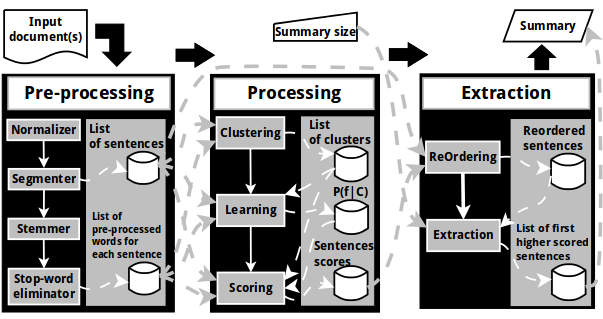
\includegraphics{mine/gnrl-arch.pdf}
\caption{L'architecture générale de notre système.}
\label{fig:gnrl-arch}
\end{center}
\end{figure}

Pour mieux comprendre la méthode, nous allons utiliser un texte qui va être utilisé dans tous les modules. 

\begin{kexp}
Supposant que notre texte d'entrée est composé des cinq phrases suivantes:
\begin{enumerate}
\item \textit{My name is Karim, and I study informatics at ESI, which is at Algiers, to obtain Magister degree.}
\item \textit{My research in ESI is about ATS, it is the intersection between IR and NLP.}
\item \textit{In this research, the main idea is to find relevant sentences using IR technics.}
\item \textit{The statistical features are the power of IR to find relevancy.}
\item \textit{AI technics are used, such as learning algorithms to create models for each topic in the input text.}
\end{enumerate}
\end{kexp}

\subsection{Module de pré-traitement}

Dans le module de pré-traitement, on nécessite les étapes suivantes:
\begin{itemize}
\item Segmentation des phrases en utilisant le framework OpenNLP d'Appache\footnote{Site web: \url{http://opennlp.apache.org/}}. 
\item Pour détecter les mots, on a implémenté un simple algorithme est utilisé, qui prend l'espace comme caractère de séparation. 
\item Pour la radicalisation, nous avons utilisé Porter-stemmer \footnote{\url{http://www.tartarus.org/~martin/PorterStemmer}}; une implémentation de l'algorithme de Porter \cite{97-porter} en Java.
\end{itemize}

\begin{kexp}
Le pré-traitement de l'exemple précédent donne:
\begin{enumerate}
\item \textit{karim studi informat esi algier obtain magist degre} (8 termes)
\item \textit{research esi at intersect ir nlp} (6 termes)
\item \textit{research main idea find relev sentenc ir technic} (8 termes)
\item \textit{statist featur power ir find relev} (6 termes)
\item \textit{ai technic learn algorithm creat model topic input text} (9 termes)
\end{enumerate}
\end{kexp}
%\subsection{Module de traitement}
%
%Ce module représente le le cœur d notre système, il permet d'extraire les phrases les plus pertinentes sous forme réduite.
%Ainsi, il comporte deux sous-modules: un module de réduction de phrases, et un module d'extraction. 

\subsection{Module d'extraction}

Le module d'extraction est le module le plus important dans notre système. 
Il contient la méthode proposée pour l'extraction de phrases, en essayant de maximiser la couverture des thèmes pris en charge. 
Elle contient deux étapes: l'étape d'identification des thèmes abordés dans le document, et l'étape de classification. 
Pour détecter les différents thèmes présentés dans le document, nous avons utilisé le regroupement, ici on assume que les phrases contenant des mots similaires sont des phrases de même thème. 
Dans l'étape de classification, on essaye de concevoir un modèle de chaque groupe (cluster), qui va être utilisé pour calculer la probabilité qu'une phrase appartient à un thème donné.

\subsubsection{Notre motivation}

Dans les méthodes qui utilisent le regroupement \cite{01-nomoto-al,02-hardy-al,11-song-al}, chaque thème fournit une phrase qui le représente dans le résumé; i.e. on sélectionne une phrase par thème. 
Dans ces travaux, assurer la couverture de tous les thèmes par le résumé produit pose un problème de contrôle de la taille du résumé. 
En effet, pour un résumé de 10 documents, par exemple, avec 50 thèmes identifiés et si on sélectionne une phrase associée à chaque cluster, on aura donc un résumé de 50 phrases, ce qui n'est pas du tout pratique. 
%Les thèmes négligeables par rapport au thème principal, sont souvent ignorés par ces travaux.
Le problème avec ces méthodes est que, pour tout thème identifié, on extrait une phrase correspondante malgré que, naturellement, tous les thèmes n'ont la même importance et il y en a même quelques thèmes qui sont négligeables. 
On peut trouver aussi des thèmes qui ne peuvent pas être représentés ou résumé par une seule phrase. 

L'idée principale est de sélectionner les phrases qui peuvent représenter tous ou la plupart des thèmes, en donnant à une phrase un score pour, ensuite, combiner ces scores en un score final utilisé pour l'ordonnancement des phrases.
Afin de calculer le score de chaque phrase par thème, on utilise un algorithme d'apprentissage (Naïve Bayes), pour entrainer le système sur les différents clusters et les critères. 
Contrairement aux systèmes précédents basés sur l'apprentissage \cite{95-kupiec-al,01-amini-gallinari,02-osborne,05-yeh-al,10-yatsko-al}, ce système n'a pas besoin d'un corpus d'entraînement, l'apprentissage est utilisé uniquement pour l'obtention du score par cluster. 

\subsubsection{Le regroupement}

Afin de regrouper les phrases, nous avons utilisé une mesure de calcul de la similarité entre deux segments : la similarité Cosinus. Cette mesure a été largement appliquée dans le domaine de la recherche d'information.
Ici, l'équation \ref{eq:cosine-g} est utilisé pour calculer la similarité Cosinus entre deux phrases $ X $ et $ Y $.
\begin{equation}
\label{eq:cosine-g}
cos(X,Y) = \frac {\sum_i {x_i.y_i} }
{\sqrt{\sum_i(x_i)^2} . \sqrt{\sum_i(y_i)^2}}
\end{equation}
Où: $ x_i $ est le mot numéro $ i $ dans la phrase $ X $, et $ y_i $ est le mot numéro $ i $ dans la phrase $ Y $.
Pour notre exemple, les deux phrases $ s_3 $ et $ s_4 $ ont les termes \{ir, find, relev\} en commun. 
Donc, $ cos(s_3,s_4)= (1*1 + 1*1 + 1*1) /(\sqrt{1^2+1^2+1^2+1^2+1^2+1^2+1^2+1^2}*\sqrt{1^2+1^2+1^2+1^2+1^2})\approx 0.43$.

Ainsi, on considère que deux phrases $ X $ et $ Y $ sont similaires, si leur similarité cosinus $ cos(X,Y) $ est supérieure à un certain seuil $ Th $.
Notre algorithme de regroupement passe par les étapes suivantes (voir la figure \ref{fig:cluster}):
\begin{figure}[ht]
\begin{center}
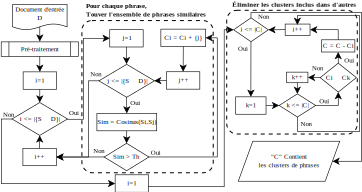
\includegraphics[width=160mm]{mine/cluster.pdf}
\caption{Algorithme de regroupement.}
\label{fig:cluster}
\end{center}
\end{figure}
\begin{itemize}
\item Pour chaque phrase, on calcule sa similarité avec toutes les autres phrases en utilisant l'équation \ref{eq:cosine-g}.

\item Ensuite, on utilise un seuil $ Th $ pour sélectionner les phrases les plus similaires. 
Si le seuil est élevé, les clusters formés vont contenir un nombre réduit de phrases. 
S'il est trop faible, les clusters seront, serte, moins nombreux et plus grands, mais en contrepartie on perd en termes de cohésion des clusters, les thèmes deviennent ainsi flous. %\cite{Clustering-Hardy-2002}

\item Chaque phrase et celles qui lui sont similaires vont construire un cluster. 

\item Nous exécutons les trois premières étapes jusqu'à ce qu'il ne reste aucune phrase. 

\item Après avoir terminé toutes les $ n $ phrases, nous obtenons $ n $ clusters (une phrase peut appartenir à plusieurs clusters). 

\item Pour chaque cluster, on vérifie s'il n'est pas inclut dans un autre cluster. Sinon, on l'efface. 

\item Enfin, on obtient un nombre total de clusters inférieur ou égal au nombre de phrases.

\end{itemize}

\begin{kexp}
Prenant notre exemple précédent, en suivant les étapes de notre algorithme, on aura:
\begin{itemize}
\item Les similarités entre les cinq phrases sont: $ cos(s_1,s_2) \approx 0.14$, $ cos(s_1,s_3) = cos(s_1,s_4) = cos(s_1,s_5) =0.0 $, $ cos(s_2,s_3) \approx 0.29 $, $ cos(s_2,s_4) \approx 0.17 $, $ cos(s_2,s_5) =0.0 $, $ cos(s_3,s_4) \approx 0.43 $, $ cos(s_3,s_5) \approx 0.12 $, et $ cos(s_4,s_5) \approx 0.0 $.

\item Prenant la valeur $ Th=0.2 $.

\item On aura les clusters suivants: $ C_1 = \{s_1\} $, $ C_2 = \{s_2, s_3\} $, $ C_3 = \{s_2, s_3, s_4\} $, $ C_4 = \{s_3, s_4\} $, $ C_5 = \{s_5\} $.

\item On remarque que le cluster $ C_2 $ est inclus dans le cluster $ C_3 $, et le cluster $ C_4 $ est inclus dans le cluster $ C_3 $.

\item Après suppression et ré-ordonnancement de clusters, on aura $ C_1 = \{s_1\} $, $ C_2 = \{s_2, s_3, s_4\} $, $ C_3 = \{s_5\} $.

\end{itemize}
\end{kexp}

\subsubsection{La fonction de score en utilisant la classification}

Dans le but de rendre notre méthode aussi générale que possible, nous avons choisi de ne pas utiliser un corpus d'apprentissage, et plutôt, nous utilisons différents clusters pour le faire.
Supposant que nous avons des clusters de phrases similaires. 
Dans notre méthode, nous voulons trouver les phrases qui sont les plus probables pour représenter tous les clusters. 
Ceci peut être représenté par l'équation suivante: 
\begin{equation}
\label{eq:sent-score}
P(s_i \in \bigcap_{j} C_j | \overrightarrow{f}) = 
\prod_{j} P(s_i \in C_j | \overrightarrow{f})
\end{equation}
Où $s_i$ est la phrase numéro $i$, $C_j$ est la classe $j$, et $\overrightarrow{f}$ est le vecteur de critères (fréquence de mots, longueur de phrase, position de phrase, etc.).

Pour calculer la probabilité qu'une phrase $s_i$ appartient à une classe $C_j$ sachant un vecteur de critères $\overrightarrow{f}$, nous avons utilisé la classification de Bayes. 
Si nous supposons l'indépendance de critères et, en utilisant la théorème de Bayes, nous avons:
\begin{equation}
\label{eq:bayes}
P(s_i \in C_j | \overrightarrow{f}) = 
\frac{P(s_i \in C_j) . P(\overrightarrow{f} | s_i \in C_j) }{P(\overrightarrow{f})}
\end{equation}
Puisque le dénominateur ne dépend pas des classes et les valeurs des critères (constant), l'équation \ref{eq:bayes} s'écrit:
\begin{equation}
\label{eq:bayes2}
P(s_i \in C_j | \overrightarrow{f}) \propto 
P(s_i \in C_j) . P(\overrightarrow{f} | s_i \in C_j)
\end{equation}
De l'équation \ref{eq:sent-score} et \ref{eq:bayes2}, on obtient l'équation suivante:
\begin{equation}
\label{eq:bayes3}
P(s_i \in \bigcap_{j} C_j | \overrightarrow{f}) \propto 
\prod_{j} P(\overrightarrow{f} | s_i \in C_j)
\end{equation}
Car nous multiplions toutes les probabilités a priori ($P(s_i \in C_j)$), le résultat peut être supprimée puisqu'elle est constante. 
En revanche, Bayes suppose l'indépendance de critères les uns des autres, et donc l'équation \ref{eq:bayes3} peut être écrite comme suit:
\begin{equation}
\label{eq:bayes4}
P(s_i \in \bigcap_{j} C_j | \overrightarrow{f}) \propto 
\prod_{j} \prod_{k} P(f_k | s_i \in C_j)
\end{equation}

Pour faciliter la combinaison des différents critères d'une phrase, en particulier ceux de la fréquence du terme, nous proposons d'utiliser un score plutôt qu'une probabilité. 
Un autre raison est que la classification utilisée ici n'est qu'un outil de score (donner des scores à une phrase dans chaque cluster), et pas la construction d'un modèle qui permet de définir les phrases de résumé ou de régler les poids des critères. 
Alors, l'équation \ref{eq:bayes4} va être écrite comme suit:
\begin{equation}
\label{eq:class-score}
Score(s_i , \bigcap_{j} C_j , \overrightarrow{f}) = 
\prod_{j} \prod_{k} Score(s_i , C_j , f_k )
\end{equation}
Enfin, les phrases vont être réorganisées selon leurs scores. 
La fonction $ Score( s , C , f ) $ est utilisée pour calculer le score de la phrase $ s $ dans la classe $ C $, en utilisant le critère $ f $ qui peut apparaître plusieurs fois dans cette phrase. 

Ensuite, on passe à l'échelle de logarithme, et la formule \ref{eq:class-score} devienne:
\begin{equation}
\label{eq:log-class-score}
Score_{log}(s_i , \bigcap_{j} C_j , \overrightarrow{f}) = 
\sum_{j} \sum_{k} log (Score(s_i , C_j , f_k ))
\end{equation}
Il est à noter que l'application du logarithme ne change pas l'ordre des scores, elle nous permet seulement de réduire l'espace des valeurs.

\subsubsection{L'apprentissage}

Pendant la tâche d'apprentissage, la probabilité qu'un critère apparaît dans une classe est donnée par l'équation \ref{eq:likelihood}.
Où $\phi$ est l'observation de le critère $ f $ dans la classe $ C $. 
$F_{C\phi}$ est le nombre d'apparition de $\phi$ dans la classe $ C $.
\begin{equation}
\label{eq:likelihood}
P(f = \phi | C) = \frac {F_{C\phi}}{\sum_{\phi'}{F_{C\phi'}}}
\end{equation}
et ainsi,
\begin{equation}
\label{eq:sum_likelihood}
\sum_{\phi} P(f = \phi | C) = 1
\end{equation}
Le score d'une phrase $ s $ dans une classe $ C $ en utilisant un critère $ f $,peut être représenté comme la somme des probabilités des observations de $ f $.
Ensuite, on ajoute un à la somme pour éviter la multiplication par un score d'un critère égal à zéro.
\begin{equation}
\label{eq:score}
Score(s , C , f ) = 1 + \sum_{\phi \in s} {P(f=\phi | s \in C)}
\end{equation}

\begin{kexp}
Dans notre exemple, nous allons utiliser les deux critères: les uni-grammes et les bi-grammes. 
Les statistiques de chaque cluster (ou class) seront:
\begin{itemize}
\item $\mathbf{C_1 = \{s_1\}} $:\\
\textbf{uni}=\{degre=1, magist=1, algier=1, obtain=1, informat=1, karim=1, esi=1, studi=1\}.\\
\textbf{bi}=\{informat?esi=1, karim?studi=1, >>?karim=1, magist?degre=1, studi?informat=1, algier?obtain=1, obtain?magist=1, esi?algier=1\}.

\item $ \mathbf{C_2 = \{s_2, s_3, s_4\}} $:\\
\textbf{uni}=\{ir=3, idea=1, technic=1, relev=2, esi=1, at=1, research=2, statist=1, main=1, sentenc=1, featur=1, power=1, nlp=1, itersect=1, find=2\}.\\
\textbf{bi}=\{idea?find=1, find?relev=2, itersect?ir=1, power?ir=1, ir?nlp=1, main?idea=1, >>?research=2, research?esi=1, sentenc?ir=1, research?main=1, featur?power=1, >>?statist=1, esi?at=1, ir?technic=1, relev?sentenc=1, at?itersect=1, statist?featur=1, ir?find=1\}.\\

\item $ \mathbf{C_3 = \{s_5\}} $:\\
\textbf{uni}=\{topic=1, text=1, input=1, model=1, ai=1, technic=1, creat=1, learn=1, algorithm=1\}.\\
\textbf{bi}=\{input?text=1, technic?learn=1, creat?model=1, algorithm?creat=1, >>?ai=1, model?topic=1, topic?input=1, learn?algorithm=1, ai?technic=1\}.
\end{itemize}

Maintenant, calculons la probabilité de l'occurrence "ir" de critère "uni-grammes" dans le deuxième cluster $ P(f = "ir" | C_2) $. 
$ P(f = "ir" | C_2) = 3/(3+1+1+2+1+1+2+1+1+1+1+1+1+1+2) = 3/20 = 0.15$. 
Pour simplifier le calcul, et puisque le nombre des occurrences de critères dans les clusters vont être multiplié qui nous donne un nombre constant, nous allons prendre $ P(f = "ir" | C_2) = 3 $.

pour chaque phrase, on calcule son score dans un cluster $ C $ avec un critère $ f $ en utilisant l'équation \ref{eq:score}. 
Le score de la phrase $ s_3 $ dans le cluster $ C_2 $ avec le critère "uni-grammes" sera: 
$ Score(s_3 , C_2 , uni ) = 1 + (2 + 1 + 1 + 2 + 2 + 1 + 3 + 1) = 14 $. 
De même, on aura:
\begin{enumerate}
\item $ Score(s_1 , C_1 , uni ) = 9 $, $ Score(s_1 , C_1 , bi ) = 9 $, 
$ Score(s_1 , C_2 , uni ) = 2 $, $ Score(s_1 , C_2 , bi ) = 1 $, 
$ Score(s_1 , C_3 , uni ) = 1 $, $ Score(s_1 , C_3 , bi ) = 1 $.

\item $ Score(s_2 , C_1 , uni ) = 2 $, $ Score(s_2 , C_1 , bi ) = 1 $, 
$ Score(s_2 , C_2 , uni ) = 10 $, $ Score(s_2 , C_2 , bi ) = 8 $, 
$ Score(s_2 , C_3 , uni ) = 1 $, $ Score(s_2 , C_3 , bi ) = 1 $.

\item $ Score(s_3 , C_1 , uni ) = 1 $, $ Score(s_3 , C_1 , bi ) = 1 $, 
$ Score(s_3 , C_2 , uni ) = 14 $, $ Score(s_3 , C_2 , bi ) = 11 $, 
$ Score(s_3 , C_3 , uni ) = 2 $, $ Score(s_3 , C_3 , bi ) = 1 $.

\item $ Score(s_4 , C_1 , uni ) = 1 $, $ Score(s_4 , C_1 , bi ) = 1 $, 
$ Score(s_4 , C_2 , uni ) = 11 $, $ Score(s_4 , C_2 , bi ) = 8 $, 
$ Score(s_4 , C_3 , uni ) = 1 $, $ Score(s_4 , C_3 , bi ) = 1 $.

\item $ Score(s_5 , C_1 , uni ) = 1 $, $ Score(s_5 , C_1 , bi ) = 1 $, 
$ Score(s_5 , C_2 , uni ) = 2 $, $ Score(s_5 , C_2 , bi ) = 1 $, 
$ Score(s_5 , C_3 , uni ) = 10 $, $ Score(s_5 , C_3 , bi ) = 10 $.

\end{enumerate}

En utilisant l'équation \ref{eq:log-class-score} et ces scores, on peut calculer le score total de chaque phrase. 
Pour chaque phrase, on aura les scores suivants: $ Score(s_1) \approx 5.09 $, $ Score(s_2) \approx 5.08 $, $ Score(s_3) \approx 5.73 $, $ Score(s_4) \approx 4.48 $, $ Score(s_5) \approx 5.30 $.
\end{kexp}

\subsubsection{La normalisation}

En utilisant le score dans l'équation \ref{eq:class-score}, les phrases dont la taille est petite, sont toujours défavorisées, et donc n'ont pas une grande chance contre celles de grande taille. 
En plus, en utilisant la réduction de phrases et en comparant les phrases réduites avec celles originales, ces dernières sont toujours favorisées.
Pour résoudre ce problème, le score peut être normalisé sur la taille du phrase en nombre de termes. 
L'équation \ref{eq:class-score} va, donc, être écrite comme suite:
\begin{equation}
\label{eq:score-norm}
Score_{norm}(s_i , \bigcap_{j} C_j , \overrightarrow{f}) = 
\frac{1}{|s_i|}
\prod_{j} \prod_{k} Score(s_i , C_j , f_k )
\end{equation}
Où: $ |s_i| $ est le nombre de termes dans la phrase $ s_i $.

En utilisant le logarithme, cette équation peut être écrit comme suit:
\begin{equation}
\label{eq:score-norm-log}
Score_{norm+log}(s_i , \bigcap_{j} C_j , \overrightarrow{f}) = 
Score_{log}(s_i , \bigcap_{j} C_j , \overrightarrow{f}) - log(|s_i|)
\end{equation}
Pour garantir que la longueur $ |s_i| $ ne soit pas à 0, on va ajouter 1. 

\begin{kexp}
Les scores de notre exemple vont être: 
\begin{enumerate}
\item $ Score_{norm}(s_1) = 5.09 - log(9) \approx 2.89 $,
\item  $ Score_{norm}(s_2) = 5.08 - log(7) \approx 3.13 $, 
\item  $ Score_{norm}(s_3) = 5.73 - log(9) \approx 3.53 $, 
\item  $ Score_{norm}(s_4) = 4.48 - log(7) \approx 2.53 $, 
\item  $ Score_{norm}(s_5) = 5.30 - log(10) \approx 3.0 $.
\end{enumerate}
\end{kexp}

\subsection{Module de compression}

%La réduction dans le premier module se fait avant l'extraction. % d'une façon similaire de \cite{07-zajic-al}. 
Pour chaque phrase de texte, on cherche la phrase compressée si elle existe. 
À la fin, nous allons avoir un nombre sa forme compressée inférieur ou égale au nombre de phrases du texte. 
Elles vont ensuite recevoir un score tout comme les phrases originale, mais elles ne participent pas dans les statistiques, puisque leurs phrases originales l'ont déjà fait. 
Dans une première fois, nous avons utilisé un algorithme très primitif pour compresser les phrases, seulement pour voir l'effet de réduction sur les résumés, et si ce chemin mérite d'être suivi ou non.
En voyant d'une façon technique à la réduction de phrases, nous ne supprimons que les expressions d'explication dont la pattern est comme suite:
\begin{itemize}
\item , which [\textasciicircum,]*,
\item , who [\textasciicircum,]*,
\item \_ [\textasciicircum\_]* \_
\end{itemize}

La première phrase "\textit{My name is Karim, and I study informatics at ESI, which is at Algiers, to obtain Magister degree.}" peut être compressée en utilisant cet algorithme, en éliminant le passage "\textit{, which is at Algiers,}". 
Le score normalisé de la phrase compressée sera $ Score(s_{1-reduit}) \approx 2.64 $. 
Dans cet exemple, la réduction n'a pas amélioré le score de la phrase 1.
%La réduction de phrases nous permet d'ajouter d'autres informations au résumé, et d'éliminer l'information non nécessaire. 
%Lorsque nous avons évalué la réduction, nous avons trouvé qu'elle peut améliorer un peu de la qualité de résumé, portant elle est si simple. 
%Cela nous encourage d'utiliser un module plus évolué dans le futur.

\subsection{Module de post-traitement}

Étant donné que notre but est, dans un premier temps, d'améliorer la qualité en termes contenu informationnel du résumé résultant, et non pas sa représentation, l'ordre des phrases, la résolution des anaphores, et l'enchaînement des idées entre les phrases font partie des perspectives de notre travail.

Concernant le problème de redondance d'information, nous avons utilisé la similarité entre phrases pour éliminer les phrases redondante du résumé. 
Ça nous permet d'avoir plus d'information dans notre résumé. 
Les étapes suivantes décrivent l'algorithme suivi afin d'éliminer la redondance:
\begin{enumerate}
\item Étant donné l'ensemble des phrases ordonnées par leurs scores, ajouter la première phrase au résumé.
\item Pour chaque phrase candidate, on vérifie si le résumé a atteint sa limite.
Si c'est le cas, on s'arrête; Sinon, on continue.
\item On calcule la similarité entre la dernière phrase ajoutée au résumé et la phrase candidate. 
Si la similarité est inférieure à certaine valeur (nous avons utilisé 0.5), on l'ajoute au résumé. 
Sinon, on passe à la phrase suivante. 
\end{enumerate}
%Notre justification est que les phrases similaires vont attribuées presque le même score. 
%C'est pour cette raison, on ne fait la comparaison qu'avec la dernière phrase dans le résumé.

En ce qui concerne la résolution des anaphores, nous avions choisi d'utiliser le module de résolution des anaphores développé par le groupe NLP de l'université de Stanford "Stanford CoreNLP\footnote{Site web: \url{http://nlp.stanford.edu/software/corenlp.shtml}}" \cite{13-lee-al}.
Ce système met en œuvre une méthode de résolution d'anaphores multi-passes décrit dans \cite{11-lee-al} et \cite{10-raghunathan}.
Pour notre cas, on fait passer tous le texte par ce module pour ensuite corriger celles qui sont présente au niveau du résumé.

\section{Application au résumé multi-documents}

\subsubsection{Résumé en utilisant les documents comme clusters}

La première méthode consiste à considérer chaque document en entrée comme un cluster de phrases pour ensuite appliquer l'algorithme d'apprentissage sur chaque document à part. 
En deuxième lieu, chaque modèle est utilisé pour la notation de phrases des documents d'entrée.
La figure \ref{fig:system1} illustre les différentes étapes de cette méthode. 
%
\begin{figure}[!ht]
\begin{center}
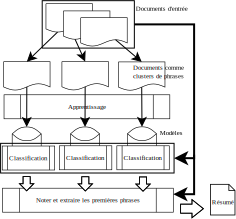
\includegraphics[width=100mm]{mine/system1.pdf} %[width=100mm]
\caption{Architecture du système en utilisant chaque document comme cluster.}
\label{fig:system1}
\end{center}
\end{figure}

Dans cette architecture, chaque cluster est un document d'entrée. 
Le problème est que les documents d'entrée ont le même thème général, et des thèmes secondaires qui peuvent être différents d'un document à l'autre. 
Donc, l'algorithme d'apprentissage va générer des modèles qui sont très proches. 
Cela nous conduit d'utiliser une autre méthode qui nous permet de traiter des clusters plus distinctifs.

\subsubsection{Résumé par fusion de documents}

La deuxième méthode consiste à fusionner tous les documents d'entrée, en les considérant comme un seul document. 
Ainsi, on regroupe les phrases similaires dans le même cluster. 
Ensuite, on applique l'algorithme d'apprentissage sur les clusters de phrases pour obtenir un modèle pour chacun. 
Finalement, chaque modèle est utilisé pour donner un score pour chaque phrase des documents d'entrée.
La figure \ref{fig:system2} illustre les différentes étapes de cette méthode. 
%
\begin{figure}[!ht]
\begin{center}
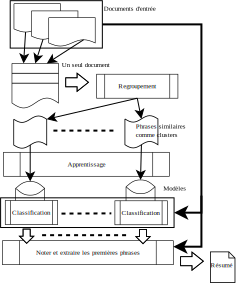
\includegraphics[width=100mm]{mine/system2.pdf} %[width=100mm]
\caption{Architecture du système en fusionnant les documents.}
\label{fig:system2}
\end{center}
\end{figure}

\section{Conclusion}

Dans ce chapitre, nous avons présenté notre système de résumé automatique de textes. 
Premièrement, nous avons présenté l'architecture générale utilisée par les systèmes de résumé automatique, en spécifiant les différents modules, ainsi que la description de chaque module dans notre système.
Le module, au cœur systèmes d'extraction, est le module d'extraction. 
Dans notre système, ce module utilise deux techniques: le regroupement pour trouver les différents thèmes de document(s), et la classification pour donner un score à chaque phrase. 
Ainsi, nous avons présenté l'algorithme de regroupement que nous avons utilisé pour définir des clusters contenant les phrases ayant le même thème. 
Ensuite, nous avons discuté l'utilisation de la classification pour trouver les phrases pertinentes sans avoir besoin d'un corpus d'entraînement. 
Ces deux techniques sont utilisées dans le résumé mono-document, en utilisant les clusters résultants de regroupement comme entrée au système d'apprentissage pour mesurer la pertinence des phrases par rapport à tous les thèmes de texte. 
Nous avons présenté deux approches pour le résumé multi-documents: la première prend chaque document comme cluster de phrases, et la deuxième fusionne les différents documents. 

Notre méthode de regroupement est utilisée pour détecter les différents thèmes de document(s), d'une manière simple et rapide, afin de tester l'effet du regroupement sur le système de résumé. 
On peut utiliser d'autres méthodes de regroupement plus évolués, pour assurer une identification plus précise des différents thèmes de texte. 
En ce qu concerne la classification, nous avons choisi le classificateur Naïve Bayes, qui est simple à modéliser et qui a prouvé son utilité pour le résumé automatique à base d'apprentissage. 
%On peut toujours tester d'autres algorithmes de classification, ce qu'il n'est pas notre but dans ce travail. 

Dans le chapitre suivant, nous allons présenter les différentes évaluations conduites sur notre système. 
Nous allons évaluer l'effet des seuils de regroupement sur le résumé résultant, ainsi que l'effet d'ajout de critères. 
Enfin, on va comparer notre système avec d'autres systèmes de résumé automatique de texte. 

\ifx\wholebook\relax\else
 %\chapterfoot
 \cleardoublepage
 \bibliographystyle{../use/ESIbib} 
 \bibliography{../bib/mine} 
 \end{document}
\fi
